%\setcounter{page}{1}
\setcounter{equation}{0}
\setcounter{figure}{0}

\section{Where's the Electron?}

Name \rule{2.0in}{0.1pt}\hfill{}Section \rule{1.0in}{0.1pt}\hfill{}Date
\rule{1.0in}{0.1pt}

\textbf{Objective}

To solve the Schroedinger equation for the hydrogen atom,
use the results to visualize the probability distribution of the electron, and to
determine the location of the electron as a function of energy, radeial position, angle, 
and angular momentum.

\textbf{Apparatus}

\begin{itemize}

\item {\it Schr\"odinger Shooter} software

\item {\it Mathematica}.

\end{itemize}

\textbf{Overview}

Quantum mechanics is the theoretical structure used to understand the atomic and sub-atomic
world. 
We start with the three-dimensional
energy of a particle in a Coulomb field that can be written as
\begin{equation}
E = \frac{p_r^2}{2m} + \frac{L^2}{2mr^2} - k_e\frac{e^2}{r}
\end{equation}\label{eq:probdens1}
\noindent where $r$ is the distance from the proton to the electron in the hydrogen atom,
$m$ is the electron mass, $p_r$ is the radial component of the momentum, 
$e$ is the electronic charge, $k_e$ is the Coulomb constant, and
$L$ is the angular momentum.
The energy only depends on $r$ and $p_r$.
The first two terms form the kinetic energy and the third term is the potential energy.
The angular momentum $L$ is a constant of the motion so the last two terms in 
Equation 1 above can be treated as a single `effective' potential 
that governs the radial motion of particle.
This form of the energy is then used to assemble a set of postulates that form
the basis of the quantum theory.

\begin{center}
{\bf The Postulates of Quantum Mechanics}
\end{center}

\begin{enumerate}

\item The quantum state of a particle is characterized by a wave function  
$\Psi(\vec r,t)$, which contains all the information about the system an observer can 
possibly obtain.
The square of the magnitude of the wave function $|\Psi (\vec r,t)|^2$ 
is interpreted as a probability or probability density of the particle's location. 

\item The things we measure ({\it e.g.} energy, momentum) are called observables. 
Each observable has a corresponding mathematical object called an operator 
that does `something' to the wave function $\Psi(\vec r,t)$.
The radial dependence of the wave function $\Psi(\vec r,t)$ is governed by
the energy operator which generates an expression called the
Schr\"odinger equation.
\begin{equation}
-\frac{\hbar^2}{2 m}\left ( \frac{d^2}{d r^2} +  
   \frac{L^2}{2 m r^2} \right ) \Psi(r) + U \Psi(r) = E  \Psi(r)
\end{equation}\label{eq:probdens2}
\noindent In this laboratory, the potential energy $U$ will be the Coulomb potential energy $U_C = -k_e e^2/r$
(see Equation 1).

\end{enumerate}

\textbf{Activity 1: The Electron Potential Energy}

(a) Make a sketch of the potential energy as a function of $r$.
Make sure you label your axes.
What are the limiting values of the potential?
\vskip 4.0cm

\newpage

(b) The angular momentum $L$ is a constant of the motion so the last two terms in 
Equation 1 can be treated as a single `effective' potential 
that governs the radial motion of particles.
Make a sketch of those last two terms as a function of $r$ for constant $L$
as a dashed line on the same sketch you made in part 1.a.
How is your curve different from the one in 1.a?
\vskip 2.0cm


(c) Make a sketch of those last two terms similar to the one in part 1.b, but with a larger
value of the angular momentum $L$.
Use a dotted line to add the curve to your previous drawing.
How is your curve different from the one in 1.b?
\vskip 2.0cm


(d) Since the total energy is constant you can draw it on your previous sketch as a flat, straight
line. We are considering bound states (the hydrogen atom) so $E < 0$.
Draw an energy line for a bound state on your previous sketch.
Does your energy `curve' intersect the effective potential curve anywhere?
For a classical particle like a ball rolling on a hill or a satellite orbiting the
Earth,
what happens at this intersection?
Describe the motion of a classical particle in this potential.
What restrictions are there on the energy $E$ of a classical particle?
\vskip 3.0cm

\textbf{Activity 2: Quantum Predictions}

(a) What do you expect the probability distribution $|\psi|^2$ 
of the electron in a hydrogen atom to look like?
Make a sketch of your prediction.
Consider what happens
as the effective potential changes with $r$.
Be sure to label your axes.
\vskip 4.0cm

\newpage

(b) What do you expect for the probability distribution as the energy increases?
Sketch the probability distribution at a higher energy as
a dashed line on the figure you drew in part 2.a.
How is it different from the curve you made in 2.a?
\vskip 4.0cm

(c) What do you expect for the  probability distribution if the energy is fixed, but the
angular momentum increases?
Sketch this probability distribution function as
a dotted line on the figure you drew in part 2.a.
How is it different from the curve you made in 2.b?
\vskip 4.0cm

\textbf{Activity 3: Solving the Schr\"odinger Equation}

(a) We are now ready to start solving the Schr\"odinger Equation.
Go first to the {\tt All Programs} menu, then
to {\tt Physics Applications} and click on {\tt Shooter}.
You will see the {\tt Schr\"odinger Shooter} window like the one in the next figure.
If you don't see this window, consult your instructor.
\begin{figure}[hbt]
\begin{center}
\includegraphics[width=5.0in]{qmProbability/shooter1b.eps}
\caption{Initial panel for {\it Schr\"odinger Shooter}.}
\end{center}
\end{figure}

(b) The first step is to select a potential energy function.
Click on {\tt File} and go to {\tt New Potential Energy Function}.
Select the potential energy function most appropriate for the hydrogen atom.
Next select the charge of the atomic nucleus by entering that value in the 
box labeled {\tt Z:} in units of the electronic charge $e$.
Set the quantum number of the angular momentum to zero in the box
labeled {\tt L:}.
Use the first menu button on the left-hand side at the bottom of the {\tt Schr\"odinger Shooter}
window to choose {\tt Amplitude Squared} so the lower plot will be $|\psi|^2$.
Use the second menu button from the left-hand side of the
window to choose {\tt Normalized} wave functions (it should be labeled {\tt Not Normalized}
when you start the program).
This last choice makes it easier to compare wave functions for different quantum numbers.
Last, set the initial value of the energy to -1.5 in the box labeled 
{\tt Energy (Rydbergs):} and hit return.
The conversion between eV and rydbergs is $\rm 13.605 6923(12)~ eV/rydberg$.
The number in parentheses is the uncertainty on the last two digits in the
experimental value.
At this point you should see curves in both of the panels of the 
{\tt Schr\"odinger Shooter} window.
If you don't, consult your instructor.

(c) You should see several curves in the panels.
What quantities do the blue, light blue, red, yellow, and green curves represent?
Use the legend in the lower right portion of the {\tt Schr\"odinger Shooter}
window.
Record them here.
\vspace{2.5cm}

\newpage

\vspace{-0.2in}

(d) You can now adjust the energy of the electron in the field of the proton to find 
the energy levels of hydrogen.
There are three ways to change this energy.
There is a slide on the left-hand side of the {\tt Schr\"odinger Shooter} window.
Click and drag the slide to change the energy and read the value
in the box labeled {\tt Energy(Rydbergs)} located near the top of the 
{\tt Schr\"odinger Shooter} window.
You can also enter the energy in the same box
labeled {\tt Energy(Rydbergs):} as you did in part 3.b.
Last, to the right of this last box there are buttons labeled
{\tt Adjust Energy:} that will increase or decrease the energy and change the step size.

(e) Tune the energy to find lowest energy level in your hydrogen atom by obtaining
a physically acceptable probability distribution.
You may need to increase the horizontal range to view the full wave function.
You can do this by increasing the value in the box labeled {\tt Cutoff:} at the
bottom of the {\tt Schr\"odinger Shooter} window.
If you increase the horizontal scale, then increase the next box labeled
{\tt Count:} (next to the {\tt Cutoff} box) by the same ratio.
In other words, if you double the cutoff, then double the count.
This last parameter controls the stepsize used in the numerical integration of
the Schr\"odinger equation.
Sketch $|\psi|^2$ here when you have found the correct energy level.
What postulate did you exploit to find the correct solutions?
Where is the electron most likely to be found?
Where is the electron least likely to be found?
\vspace{2.0cm}

\newpage

(f) Next, tune the energy to find the third energy level (second excited state)
in your hydrogen atom by obtaining
a physically acceptable probability distribution.
Sketch $|\psi|^2$ here when you have found the correct energy level.
How does $|\psi|^2$ change as the energy increases?
Where is the electron most likely to be found?
Where is the electron least likely to be found?
\vspace{4.5cm}

(g) Next, change the value of the angular momentum quantum number from $l=0$
to $L=1$.
Tune the energy to find the energy level for this state.
Sketch $|\psi|^2$ when you have found the correct energy level.
How is it different from the the result in part 3.f?
Where is the electron most likely to be found?
Where is the electron least likely to be found?
Is the energy here different from the energy in part 3.f?
\vspace{4.5cm}

(h) Summarize your results here. How does the probability distribution $|\psi|^2$ 
change as the energy (and the principle quantum number $n$) increases?
How does changing the value of the angular momentum $L$ change the energy?
How does it change $|\psi|^2$?
\vspace{4.5cm}

\textbf{Activity 4: Where is the Electron?}

We will now explore the probability distribution of the electron bound to a proton as a function
of the distance $r$ from the proton to the electron and the angle $\theta$ relative to the $z$ axis.

(a) Download the {\it Mathematica} file {\it HydrogenOrbitals.nb} from the location \\
\begin{center}
{\verb!https://facultystaff.richmond.edu/~ggilfoyl/genphys/132/links.html!}
\end{center}
\noindent and store it on your computer {\tt Desktop}.

(b) Go to the {\tt All Programs} menu and click on {\tt Mathematica}.
You should see {\it Mathematica} go through its startup and then click {\tt Open}
on the {\it Mathematica} start-up screen.
Locate the file you just downloaded and open it.
Follow the instructions in the {\it Mathematica} notebook
and you will get the interface shown below for plotting
the electron probability density for the hydrogen atom.
If you don't see the interface in Figure \ref{fig:gui}, consult your instructor.
Click on the buttons and play with the sliders to see how they effect the 
probability distribution for the hydrogen orbitals.
\begin{figure}[h!]
\begin{center}
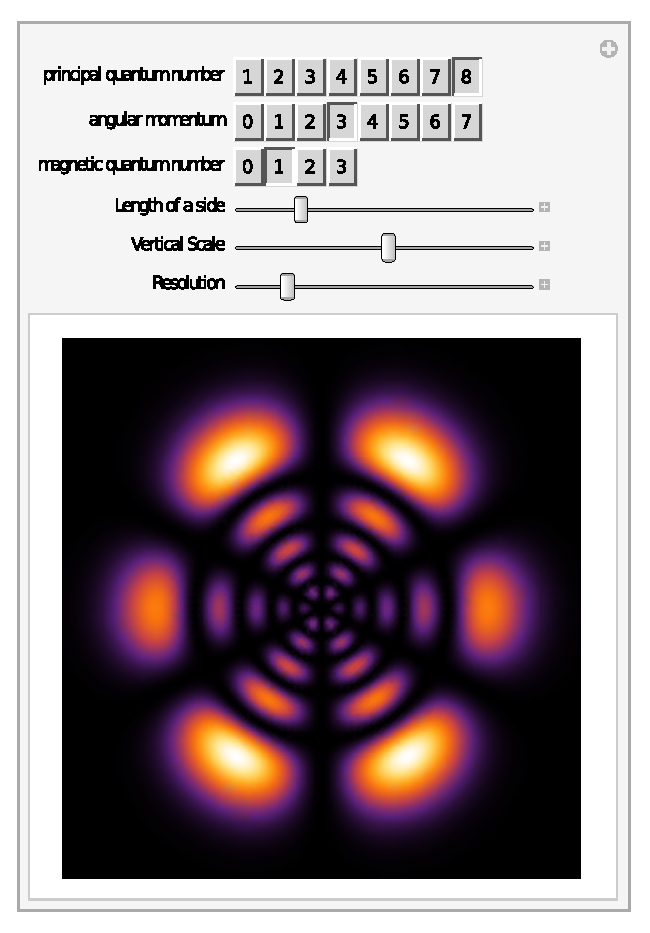
\includegraphics[width=3.0in]{qmProbability/qmPlot2.eps}
\caption{Panel for {\it HydrogenOrbitals.nb}}\label{fig:gui}
\end{center}
\end{figure}

(c) Examine different values of the principle quantum number $n$ for $L=0$.
How does $|\psi|^2$ change as $n$ increases? Compare these pictures with your results for 
$|\psi|^2$ for increasing energy in parts 2.f and 2.g.
Where is the electron most likely to be found?
Where is the electron least likely to be found?
\vspace{3.0cm}

\newpage

(d) Set the principle quantum number to $n=8$ and the angular momentum to $L=0$.
Increase the value of $L$.
Describe what happens to the probability distribution.
Where is the electron most likely to be found?
Where is the electron least likely to be found?
\vspace{3.0cm}

(e) Return to your predictions in Activity 2 and examine your predictions.
How did you do?
Correct any statements that you now find are wrong.
\vspace{2.0cm}

(f) Based on what you now know can you describe the motion of the electron
in the hydrogen atom? Explain.

\vspace{3.0cm}
